\begin{figure}[ht]\centering
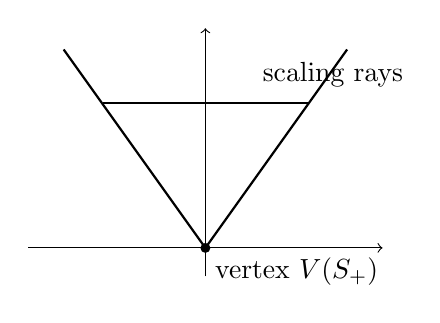
\begin{tikzpicture}[scale=.9]
\draw[->] (-2.5,0)--(2.5,0);\draw[->] (0,-.4)--(0,3.1);
\draw[thick] (-2,2.8)--(0,0)--(2,2.8);
\draw[thick] (-1.45,2.05)--(1.45,2.05);
\fill (0,0) circle (2pt);\node[below right] at (0,0) {vertex \(V(S_+)\)};
\node at (1.8,2.45) {scaling rays};
\end{tikzpicture}
\caption{Homogeneous equations define cones stable along scaling rays.}\label{fig:vi34-08}\end{figure}